\chapter{Introduction}
\label{chap1}
It is very critical and important to cast and count votes, the electronic voting is a term used to describe the act of voting
using electronic systems. Electronic Voting Machine (EVM) is an electronic device used
for recording votes. An Electronic Voting Machine consists of
two Units first is Control Unit and second is Balloting Unit that are joined by a 5 meter cable. The candidate names and symbol are programmed in the control unit of EVM. The polling officer in-charge of the control unit will release a ballot instead of issuing a ballot paper by pressing the ballot button on the control unit. This mechanism will enable the voter to cast his vote by pressing the blue button on the balloting unit against the candidate and symbol of his choice. \cite{nikamcritical}
\begin{figure}[H]  %h=positioning
\begin{center}
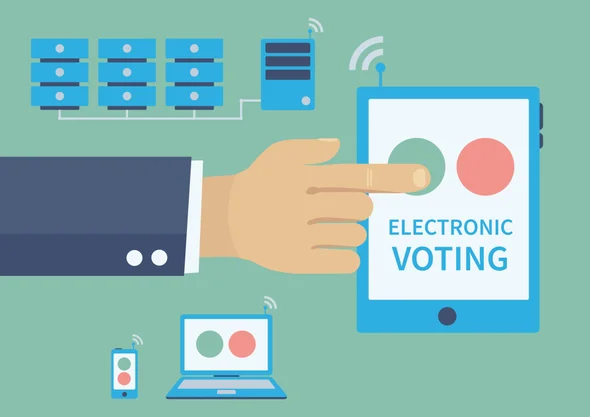
\includegraphics[scale=1.0]{Chapter1/evm}
\caption{Electronic Voting Machine (EVM)}
\label{figure1}
\end{center}
\end{figure}

\section{Objectives}
%
%
The objectives of this project are:
%
%for 1,2,3 numbers
\begin{enumerate}
\item To make elections time efficient and  cost efficient.
%
\item To eliminate the chance of rigging in the elections.
%
\item To automate the elections.
%
%
\end{enumerate}
\section{Introduction}
\noindent Elections allow the people to choose their representatives and express their preferences for how they will be governed. Naturally, the integrity of the election process is fundamental to the integrity of democracy itself. The election system must be sufficiently robust to withstand a variety of fraudulent behaviors and must be sufficiently transparent and comprehensible that voters and candidates can accept the results of an election.
Electronic voting refers to the use of computers or computerized voting equipment to cast ballots in an election. Sometimes, this term is used more specifically to refer to voting that takes place over the Internet\cite{kumar2012electronic}.

The design of a �good� voting system, whether electronic or using traditional paper ballots or mechanical devices, must satisfy a number of sometimes competing criteria.
\begin{itemize}
\item The anonymity of a voter�s ballot must be preserved
%
\item both to guarantee the voter�s safety when voting against a malevolent candidate
%
\item guarantee that voters have no evidence that proves which candidates received their votes
%
%
\end{itemize}
\begin{figure}[H]  %h=positioning
\begin{center}

\includegraphics[scale=2]{Chapter1/pic1}
\caption{EVM}
\label{figure1}
\end{center}
\end{figure}
The voting system must also be tamper-resistant to thwart a wide range of attacks, including ballot stuffing by voters and incorrect tallying by insiders. Another factor, as shown by the so-called �butterfly ballots� in the Florida 2000 presidential election, is the importance of human factors. A voting system must be comprehensible to and usable by the entire voting population, regardless of age, infirmity, or disability. Providing accessibility to such a diverse population is an important engineering problem and one where, if other security is done well, electronic voting could be a great improvement over current paper systems. Flaws in any of these aspects of a voting system, however, can lead to indecisive or incorrect election results.\cite{kohno2004analysis}


\section{E-Voting Systems}
It is also known as e-voting is a term encompassing several different types of voting, embracing both electronic means of casting a vote and electronic means of counting votes. Electronic voting technology can include punched cards, optical scan voting systems and specialized voting kiosks (including self-contained direct-recording electronic voting systems, or DRE). It can also involve transmission of ballots and votes via telephones, private computer networks, or the Internet. And, of course, EVM helps maintain total voting secrecy without the use of ballot papers. And, at the end of the polling, just press a button and
there you have the results.\cite{kumar2012electronic}


\section{Challenges}
\noindent The challenges are even harder because there is little or no training available for voters. The first time most voters ever touch the voting system is the moment they vote. And once they start voting, there is tremendous social pressure to do it without help. With people watching, inadequately trained poll workers, busy people waiting on line, the social importance of voting, and the value placed on secrecy, voters may become anxious and afraid to ask for help. Finally, the systemic issues of how voting machines get purchased and evaluated are problematic as well. State or county purchasers are usually more concerned about cost than usability. And once the systems are purchased, the public has no access to the machines for evaluation. Election workers who design ballots tend not to have experience in usability and screen design. Poll workers who deploy the voting systems have minimal training to cope with the inevitable problems. Electronic voting systems offer promise as well � from the opportunity to change font size and language on demand, to offering disabled users customized access, to accurate and fast recording and tabulation of votes. But there are many issues that add up to the risk that voters may become disenfranchised. And this is especially true for the elderly
and citizens at the margins of society.\cite{bederson2003electronic}

\subsection{Accountability and Verifiability}
Traditionally, votes were cast on paper and counted by hand. Voters were confident that the marks they made on ballots reflected their intended vote. Voting machines that used levers and punch card systems also provided voters with a high degree of confidence that they cast their votes as intended. In 2000, the U.S. presidential election was particularly contentious because the outcome was extremely close. This resulted in a close examination of the voting and tabulation systems that were used. Many problems were found, especially with one ballot design which became known as the �butterfly� ballot. This ballot required voters to draw line connecting a candidate with a circle. This was confusing because the circles didn't align well with the candidates and in addition, the circles were shared between two columns of candidates. The ensuing melee brought a popular awareness of the complexities and flaws in voting systems and there were general calls for reform. Many questions have since been raised.
Because they are paperless, systems raise the question:
 %for 1,2,3 numbers
\begin{enumerate}
\item How can one know that when a voter chooses a particular candidate on the screen?
%
\item Is a vote for that candidate is recorded?
%
\end{enumerate}
A simple solution to this problem is to provide the user with a printed record of the votes electronically recorded. Before leaving the polling place, the voter would be required to certify the contents of the paper record and place it into a ballot box. The printed records could then be manually counted in the event of a challenge, and this procedure would foil any attempt at falsifying votes
internally to the voting system. This approach, however, has not been implemented in any commercial systems that we are aware of\cite{bederson2003electronic}.

%\section{Motivation}
%Motivated by the emergence of technological advancements and challenges in ...


%
%

%
%\section{UN Stainability Goals}

 %Goal 8 is shown which is Promote sustained, inclusive and sustainable economic growth, full and productive employment and decent work for all. As we will also discuss the economical long time benefits in next chapters. Our project will help industry in economic growth as well as it is providing a help to the meter readers.



%The conceptual frame work for the proposed method is comprises of three basic building blocks and detailed model is shown in Fig. \ref{fw}.
%\begin{enumerate}
%\item Network Formation Block.
%\item Neighbourhood Based Network Matrix Formation Block.
%\item Consensus Formation Block.
%\end{enumerate}
%
%In the network formation block, ...
%
%\FloatBarrier
%\begin{figure}[H]
%\begin{center}
%\hspace{15mm}
%\includegraphics[scale=0.35]{Chapter1/robocanesinternalstates}
%
%\protect\caption{Pseudo-code of Proposed Scheme for Cooperative Control of Networked Multi-Agent Systems.}
%\label{scode}
%\end{center}
%\end{figure}
%
%
\section{Report Break Down}
%
%This thesis deals with convergence analysis .... The main contributions of this work are summarized as follows:
%
%\begin{enumerate}
%\item  Initially a design ....
%
%\item An extended ....
%
%
%\item Modeled a ....
%
%\end{enumerate}
%
%The main contribution of this work is to propose a new way ....
%
%
%
%
%\section{Thesis Outline}
%
%
The major focus of this report is on the findings of the proposed project i.e. Electronic Voting Machine(EVM) Using 8051 Microcontroller.\\

\noindent This Report is organized as follows:
\vspace{5mm}

\noindent In chapter 2, literature review is provided in detail about the work which is already been done on Electronic Voting Machine(EVM) Using 8051 Microcontroller and will give a brief details about the articles, papers and literature review.
\vspace{5mm}


\noindent In Chapter 3, Proposed Methodology is presented in which you will be able to see the method we will work on the designing of a complete project source code to the diagrams.

\vspace{5mm}


\noindent In Chapter 4, Result and Simulations are being discussed, in which you will see all kind of finding related to the Electronic Voting Machine(EVM) Using 8051 Microcontroller.


\vspace{5mm}

\noindent In Chapter 5, we have concluded and summarized the project work and also presented few new research ideas for future studies.


%\begin{equation}
%F=\sum_{n=0}^i(x_i(0)-x_j(0))^2
%%stackrel[u]{v}{T}=\stackrel[u]{v}{L}+\stackrel[u]{v}{L}\underset{W\epsilon V\cap w\neq u}{\sum}\stackrel[v]{w}{L}
%\end{equation}
